\subsection{Multivariate Kalman Filter Examples}

\begin{frame}{}
   \frametitle{Multidimensional (Multivariate) Kalman Filter Examples}

   This section includes two examples:
   \begin{itemize}
       \item Vehicle location estimation using six-dimensional Kalman Filter without control input
       \item Rocket height estimation with a two-dimensional Kalman Filter with a control input
   \end{itemize}
\end{frame}

%----------------------------------
\subsubsection{Example 9: Vehicle Location Estimation}
\label{subsec:Ex9}
\begin{frame}{Example 9: Vehicle Location Estimation}
\begin{columns}
        \column{0.45\textwidth} 
        Estimating vehicle’s location on the XY plane using onboard location sensor reporting its $X$ and $Y$ coordinates. \textit{Assumption: Constant acceleration dynamics.}
        \begin{figure}
            \centering
            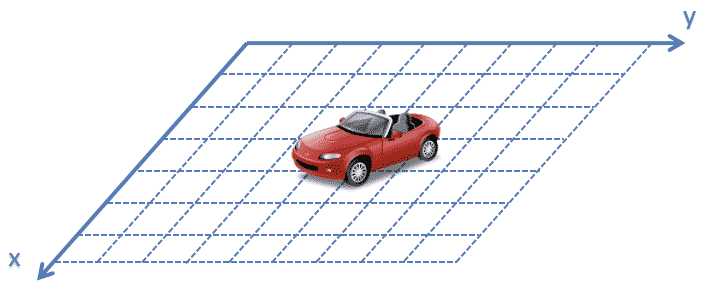
\includegraphics[width=0.7\linewidth]{Figures//Chapter3/vehicleLocationEstimation.png}
            \vspace{-5pt}
            \caption{Vehicle location estimation.}
            \label{fig:locationEstimation}
            \vspace{-5pt}
        \end{figure}
        \textbf{KF Equations}
        
        \textbf{1. The state extrapolation equation}
        \begin{equation*}
        \hat{\mathbf{x}}_{n+1,n} = \mathbf{F} \hat{\mathbf{x}}_{n,n} + \mathbf{G}\hat{\mathbf{u}}_{n,n} + \mathbf{w}_{n}
        \end{equation*}
        In this example, without control input,
        \begin{equation*}
        \hat{\mathbf{x}}_{n+1,n} = \mathbf{F} \hat{\mathbf{x}}_{n,n}
        \end{equation*}
        
        \column{0.55\textwidth}
        The system state $\mathbf{x}_n$ is defined by:
        \vspace{-7pt}
        \[
        \mathbf{x}_n =
        \begin{bmatrix}
        x_n \\
        \dot{x}_n \\
        \ddot{x}_n \\
        y_n \\
        \dot{y}_n \\
        \ddot{y}_n \\
        \end{bmatrix}
        \]
        The extrapolated vehicle state for $n + 1$ can be described as:
        \vspace{-10pt}
        \begin{align*}
\hat{x}_{n+1,n} &= \hat{x}_{n,n} + \hat{\dot{x}}_{n,n} \Delta t + \frac{1}{2} \hat{\ddot{x}}_{n,n} \Delta t^2 \\[-0.5em]
\hat{\dot{x}}_{n+1,n} &= \hat{\dot{x}}_{n,n} + \hat{\ddot{x}}_{n,n} \Delta t \\[-0.5em]
\hat{\ddot{x}}_{n+1,n} &= \hat{\ddot{x}}_{n,n} \\[-0.5em]
\hat{y}_{n+1,n} &= \hat{y}_{n,n} + \hat{\dot{y}}_{n,n} \Delta t + \frac{1}{2} \hat{\ddot{y}}_{n,n} \Delta t^2 \\[-0.5em]
\hat{\dot{y}}_{n+1,n} &= \hat{\dot{y}}_{n,n} + \hat{\ddot{y}}_{n,n} \Delta t \\[-0.5em]
\hat{\ddot{y}}_{n+1,n} &= \hat{\ddot{y}}_{n,n}
\end{align*}
\vspace{-10pt}
% Save the original array column separation
\newlength{\oldarraycolsep}
\setlength{\oldarraycolsep}{\arraycolsep}
% Reduce the space between columns
\setlength{\arraycolsep}{2pt}
\[
\begin{bmatrix}
\hat{x}_{n+1,n} \\
\hat{\dot{x}}_{n+1,n} \\
\hat{\ddot{x}}_{n+1,n} \\
\hat{y}_{n+1,n} \\
\hat{\dot{y}}_{n+1,n} \\
\hat{\ddot{y}}_{n+1,n} \\
\end{bmatrix}
=
\left[\begin{array}{@{}cccccc@{}}
1 & \Delta t & 0.5\Delta t^2 & 0 & 0 & 0 \\
0 & 1 & \Delta t & 0 & 0 & 0 \\
0 & 0 & 1 & 0 & 0 & 0 \\
0 & 0 & 0 & 1 & \Delta t & 0.5\Delta t^2 \\
0 & 0 & 0 & 0 & 1 & \Delta t \\
0 & 0 & 0 & 0 & 0 & 1 \\
\end{array}\right]
\begin{bmatrix}
\hat{x}_{n,n} \\
\hat{\dot{x}}_{n,n} \\
\hat{\ddot{x}}_{n,n} \\
\hat{y}_{n,n} \\
\hat{\dot{y}}_{n,n} \\
\hat{\ddot{y}}_{n,n} \\
\end{bmatrix}
\]
% Restore the original array column separation
\setlength{\arraycolsep}{\oldarraycolsep}
\end{columns}
\end{frame}

%-------------------------
\begin{frame}{Example 9: Vehicle Location Estimation}
\begin{columns}
        \column{0.5\textwidth} 

\textbf{2. The covariance extrapolation equation}
\begin{equation*}
\mathbf{P}_{n+1,n} = \mathbf{F}\mathbf{P}_{n,n}\mathbf{F}^T + \mathbf{Q}
\end{equation*}
The estimate covariance matrix is:
\[
\mathbf{P} =
\begin{bmatrix}
p_{x} & p_{x\dot{x}} & p_{x\ddot{x}} & p_{xy} & p_{x\dot{y}} & p_{x\ddot{y}} \\
p_{\dot{x}x} & p_{\dot{x}} & p_{\dot{x}\ddot{x}} & p_{\dot{xy}} & p_{\dot{x}\dot{y}} & p_{\dot{x}\ddot{y}} \\
p_{\ddot{x}x} & p_{\ddot{x}\dot{x}} & p_{\ddot{x}} & p_{\ddot{xy}} & p_{\ddot{x}\dot{y}} & p_{\ddot{x}\ddot{y}} \\
p_{yx} & p_{y\dot{x}} & p_{y\ddot{x}} & p_{y} & p_{y\dot{y}} & p_{y\ddot{y}} \\
p_{\dot{y}x} & p_{\dot{y}\dot{x}} & p_{\dot{y}\ddot{x}} & p_{\dot{y}y} & p_{\dot{y}} & p_{\dot{y}\ddot{y}} \\
p_{\ddot{y}x} & p_{\ddot{y}\dot{x}} & p_{\ddot{y}\ddot{x}} & p_{\ddot{y}y} & p_{\ddot{y}\dot{y}} & p_{\ddot{y}}
\end{bmatrix}
\]

Assuming the estimation errors in $X$ and $Y$ axes are uncorrelated
\[
\mathbf{P} =
\begin{bmatrix}
p_{x} & p_{x\dot{x}} & p_{x\ddot{x}} & 0 & 0 & 0 \\
p_{\dot{x}x} & p_{\dot{x}} & p_{\dot{x}\ddot{x}} & 0 & 0 & 0 \\
p_{\ddot{x}x} & p_{\ddot{x}\dot{x}} & p_{\ddot{x}} & 0 & 0 & 0 \\
0 & 0 & 0 & p_{y} & p_{y\dot{y}} & p_{y\ddot{y}} \\
0 & 0 & 0 & p_{\dot{y}y} & p_{\dot{y}} & p_{\dot{y}\ddot{y}} \\
0 & 0 & 0 & p_{\ddot{y}y} & p_{\ddot{y}\dot{y}} & p_{\ddot{y}}
\end{bmatrix}
\]

\column{0.5\textwidth} 
\textbf{}
Assuming a discrete noise model---the noise is different at each time sample but is constant between time samples.

The process noise matrix for the two-dimensional constant acceleration model looks as
\[
\mathbf{Q} =
\begin{bmatrix}
\sigma^2_x & \sigma^2_{x\dot{x}} & \sigma^2_{x\ddot{x}} & \sigma^2_{xy} & \sigma^2_{x\dot{y}} & \sigma^2_{x\ddot{y}} \\
\sigma^2_{\dot{x}x} & \sigma^2_{\dot{x}} & \sigma^2_{\dot{x}\ddot{x}} & \sigma^2_{\dot{xy}} & \sigma^2_{\dot{x}\dot{y}} & \sigma^2_{\dot{x}\ddot{y}} \\
\sigma^2_{\ddot{x}x} & \sigma^2_{\ddot{x}\dot{x}} & \sigma^2_{\ddot{x}} & \sigma^2_{\ddot{xy}} & \sigma^2_{\ddot{x}\dot{y}} & \sigma^2_{\ddot{x}\ddot{y}} \\
\sigma^2_{yx} & \sigma^2_{yx\dot{x}} & \sigma^2_{y\ddot{x}} & \sigma^2_{y} & \sigma^2_{y\dot{y}} & \sigma^2_{y\ddot{y}} \\
\sigma^2_{\dot{y}x} & \sigma^2_{\dot{y}x\dot{x}} & \sigma^2_{\dot{y}\ddot{x}} & \sigma^2_{\dot{y}y} & \sigma^2_{\dot{y}} & \sigma^2_{\dot{y}\ddot{y}} \\
\sigma^2_{\ddot{y}x} & \sigma^2_{\ddot{y}x\dot{x}} & \sigma^2_{\ddot{y}\ddot{x}} & \sigma^2_{\ddot{y}y} & \sigma^2_{\ddot{y}\dot{y}} & \sigma^2_{\ddot{y}}
\end{bmatrix}
\]
Assuming that the process noise in $X$ and $Y$ axes is not correlated:
\[
\mathbf{Q} =
\begin{bmatrix}
\sigma^2_x & \sigma^2_{x\dot{x}} & \sigma^2_{x\ddot{x}} & 0 & 0 & 0 \\
\sigma^2_{\dot{x}x} & \sigma^2_{\dot{x}} & \sigma^2_{\dot{x}\ddot{x}} & 0 & 0 & 0 \\
\sigma^2_{\ddot{x}x} & \sigma^2_{\ddot{x}\dot{x}} & \sigma^2_{\ddot{x}} & 0 & 0 & 0 \\
0 & 0 & 0 & \sigma^2_{y} & \sigma^2_{y\dot{y}} & \sigma^2_{y\ddot{y}} \\
0 & 0 & 0 & \sigma^2_{\dot{y}y} & \sigma^2_{\dot{y}} & \sigma^2_{\dot{y}\ddot{y}} \\
0 & 0 & 0 & \sigma^2_{\ddot{y}y} & \sigma^2_{\ddot{y}\dot{y}} & \sigma^2_{\ddot{y}}
\end{bmatrix}
\]
\end{columns}
\end{frame}

%-------------------------------------
\begin{frame}{Example 9: Vehicle Location Estimation}
% Columns
\begin{columns}
        \column{0.5\textwidth} 
Based on "\textcolor{blue}{How to construct $\mathbf{Q}$ matrix}" Sec.~\ref{DiscreteNoise_ConstructQMatrix}, we have:        
\[
\mathbf{Q} =
\begin{bmatrix}
\frac{\Delta t^4}{4} & \frac{\Delta t^3}{2} & \frac{\Delta t^2}{2} & 0 & 0 & 0 \\
\frac{\Delta t^3}{2} & \Delta t^2 & \Delta t & 0 & 0 & 0 \\
\frac{\Delta t^2}{2} & \Delta t & 1 & 0 & 0 & 0 \\
0 & 0 & 0 & \frac{\Delta t^4}{4} & \frac{\Delta t^3}{2} & \frac{\Delta t^2}{2} \\
0 & 0 & 0 & \frac{\Delta t^3}{2} & \Delta t^2 & \Delta t \\
0 & 0 & 0 & \frac{\Delta t^2}{2} & \Delta t & 1 \\
\end{bmatrix}\sigma_a^2
\]

where:
\begin{itemize}
    \item $\Delta t$ is the time between successive measurements
    \item $\sigma_a^2$ is a random variance in acceleration
\end{itemize}

Now Let's look at \textcolor{blue}{Auxiliary equations}:
\begin{itemize}
    \item Measurement equation
    \item Measurement uncertainty equation
\end{itemize}
        \column{0.5\textwidth}

        \textbf{Measurement equation}
        \begin{equation*}
        \mathbf{z}_n = \mathbf{H}\mathbf{x}_n + \mathbf{v}_n
        \end{equation*}

        The only measurements provided to us are $X$ and $Y$ coordinates of the vehicle.
        \[
        \mathbf{z}_n =
        \begin{bmatrix}
        x_{n,\text{measured}} \\
        y_{n,\text{measured}}
        \end{bmatrix}
        =
        \mathbf{H}
        \begin{bmatrix}
        x_n \\
        \dot{x}_n \\
        \ddot{x}_n \\
        y_n \\
        \dot{y}_n \\
        \ddot{y}_n
        \end{bmatrix}
        \]

        The dimension of $\mathbf{z}_n$ is $2 \times 1$ and the dimension of $\mathbf{x}_n$ is $6 \times 1$. Therefore, the dimension of the observation matrix $\mathbf{H}$ shall be $2 \times 6$.
        \[
        \mathbf{H} =
        \begin{bmatrix}
        1 & 0 & 0 & 0 & 0 & 0 \\
        0 & 0 & 0 & 1 & 0 & 0
        \end{bmatrix}
        \]
\end{columns}

\end{frame}


%-------------------------------------
\begin{frame}{Example 9: Vehicle Location Estimation}
% Columns
\begin{columns}
        \column{0.5\textwidth} 
        \textbf{Measurement uncertainty}
        is represented by the measurement covariance matrix:
        \[
        \mathbf{R}_n =
        \begin{bmatrix}
        \sigma^2_{x_m} & \sigma^2_{yx_m} \\
        \sigma^2_{xy_m} & \sigma^2_{y_m}
        \end{bmatrix}
        \]
        
        Assuming that the x and y measurements are uncorrelated:
        \[
        \mathbf{R}_n =
        \begin{bmatrix}
        \sigma^2_{x_m} & 0 \\
        0 & \sigma^2_{y_m}
        \end{bmatrix}
        \]
        
        In real-life applications, the measurement uncertainty can differ between measurements. In many systems, the measurement uncertainty depends on the measurement SNR, the angle between the sensor (or sensors) and target, signal frequency, and many other parameters.
        
        If we assume a constant measurement uncertainty:
        \[
        \mathbf{R}_1 = \mathbf{R}_2 = \ldots = \mathbf{R}_{n-1} = \mathbf{R}_n = \mathbf{R}
        \]
        \column{0.5\textwidth}
        \textbf{3. The Kalman Gain}
        \[
        \mathbf{K}_n = \mathbf{P}_{n,n-1} \mathbf{H}^T \left( \mathbf{H} \mathbf{P}_{n,n-1} \mathbf{H}^T + \mathbf{R}_n \right)^{-1}
        \]
        \textbf{4. The state update equation}
        \[
        \mathbf{x}_{n,n} = \hat{\mathbf{x}}_{n,n-1} + \mathbf{K}_n (\mathbf{z}_n - \mathbf{H} \hat{\mathbf{x}}_{n,n-1})
        \]
         \textbf{5. The covariance update equation}
         \[
            \mathbf{P}_{n,n} = (\mathbf{I} - \mathbf{K}_n \mathbf{H}) \mathbf{P}_{n,n-1} (\mathbf{I} - \mathbf{K}_n \mathbf{H})^T + \mathbf{K}_n \mathbf{R}_n \mathbf{K}_n^T
            \]

        
\end{columns}

\end{frame}

\begin{frame}{Example 9: Vehicle Location Estimation}
% Columns
\begin{columns}
        \column{0.5\textwidth}
        \textbf{Numerical example}: Assume a vehicle moving in a straight line in the $X$ direction with a constant velocity. After traveling 400 meters, the vehicle turns left, with a turning radius of $R=300$ meters. During the turning maneuver, the vehicle experiences acceleration due to the circular motion (angular acceleration). Recall from introductory physics that angular acceleration is given by:

        \[
        \alpha = \frac{\Delta V}{R \Delta t}
        \]


        The parameters are given as follows:

    \begin{itemize}
        \item The measurement period: \(\Delta t = 1 \, \text{s}\)
        \item The random acceleration standard deviation: \(\sigma_a = 0.2 \, \text{m/s}^2\)
        \item The measurement error standard deviation: \(\sigma_{x_m} = \sigma_{y_m} = 3 \, \text{m}\)
    \end{itemize}
    
        \column{0.5\textwidth} 
                \begin{figure}
            \centering
        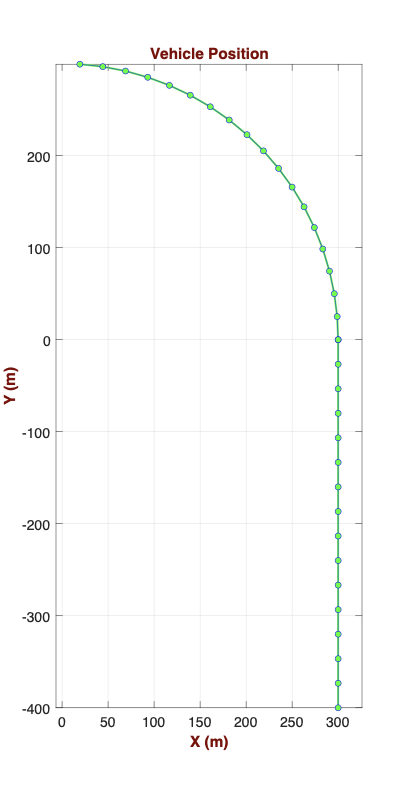
\includegraphics[width=0.6\linewidth]{Figures//Chapter3/VehiclePosition.png}
        \vspace{-12pt}
            \caption{Vehicle trajectory}
            \label{fig:VehicleTrajectory}
        \end{figure}
        
\end{columns}
\end{frame}

%----------------------------------
\begin{frame}{Example 9: Vehicle Location Estimation}
% Columns
\begin{columns}
\column{0.5\textwidth}
\vspace{-20pt}
\begin{figure}
    \centering
    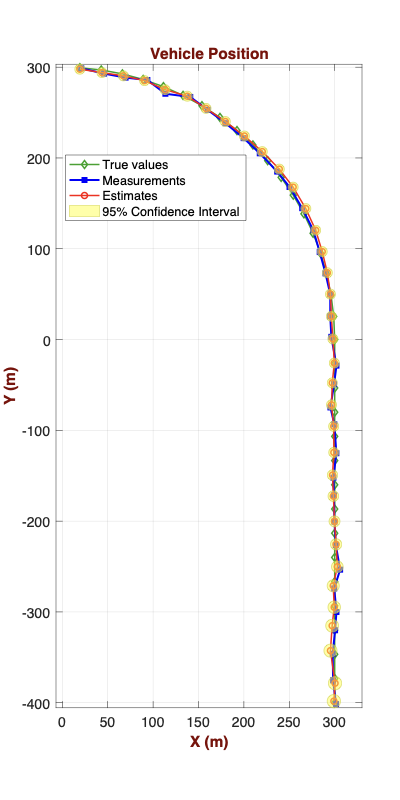
\includegraphics[width=0.5\linewidth]{Figures//Chapter3/KF_VehiclePositionEstimation.png}
    \vspace{-20pt}
    \caption{True value, measured values and estimates}
    \label{fig:KF_VehiclePositionEstimation}
\end{figure}
The circles on the plot represent the 95\% confidence ellipse. Since the $x$ and $y$ axes’
measurement errors are equal, the confidence ellipse is a circle.
\column{0.5\textwidth} 
\vspace{-15pt}
\begin{figure}
    \centering
    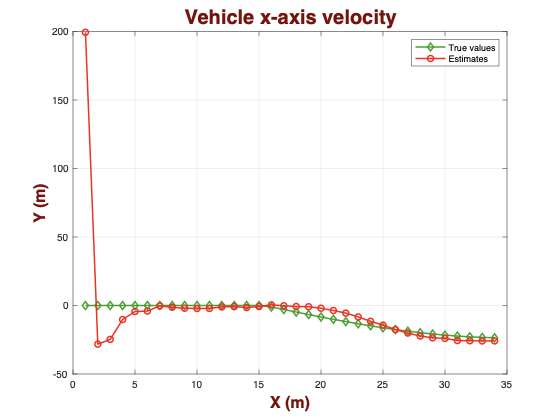
\includegraphics[width=0.9\linewidth]{Figures//Chapter3/Ex9_x_velcity.png}
    %\caption{Enter Caption}
    \label{fig:enter-label}
\end{figure}
\vspace{-15pt}
\begin{figure}
    \centering
    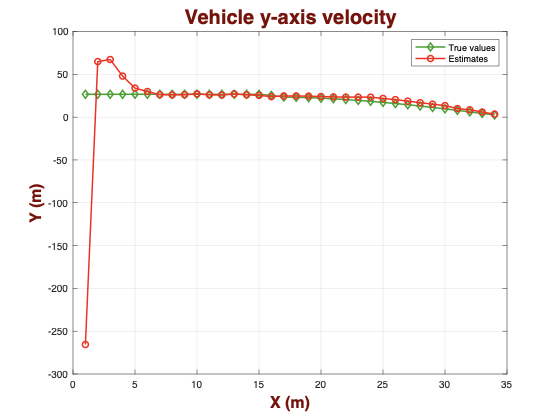
\includegraphics[width=0.9\linewidth]{Figures//Chapter3/Ex9_y_velcity.png}
    %\caption{Enter Caption}
    \label{fig:enter-label}
\end{figure}
\end{columns}
\texttt{\tiny [Code: Multivariate KF/ex9\_MultivariateKF\_LocationEstimation.m]}
\end{frame}
%----------------------------------
\subsubsection{Example 10: Rocket Altitude Estimation}
\begin{frame}{Example 10: Rocket Altitude Estimation}
\begin{columns}
\column{0.5\textwidth}
\begin{itemize}
    \item The rocket is equipped with an
onboard altimeter that provides altitude measurements.
    \item The rocket is also equipped with an accelerometer that measures the rocket’s acceleration. The accelerometer serves as a \textbf{control input to the Kalman Filter}.
    \item We assume constant acceleration dynamics.
\end{itemize}

\begin{figure}
    \centering
    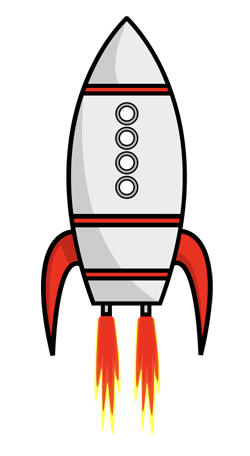
\includegraphics[width=0.35\linewidth]{Figures//Chapter3/Ex10_Rocket.png}
    \vspace{-10pt}
    \caption{Rocket altitude estimation}
    \label{fig:Rocket}
\end{figure}

\column{0.5\textwidth}
\begin{itemize}
    \item Accelerometers don’t sense gravity. An accelerometer at rest on a table measures 1g
upwards, while an accelerometer in free fall measures zero acceleration.
    \item Thus, we
need to subtract the gravitational acceleration constant $g$ from each accelerometer measurement.
\end{itemize}
 
The accelerometer measurement at time step $n$ is:

\[
a_n = \ddot{x} - g + \epsilon
\]
where:
\begin{itemize}
    \item \(\ddot{x}\) is the actual acceleration of the object (the second derivative of the object position),
    \item \(g\) is the gravitational acceleration constant; \(g = -9.8 \, \text{m/s}^2\),
    \item \(\epsilon\) is the accelerometer measurement error.
\end{itemize}
\end{columns}
\end{frame}


%----------------------------------
\begin{frame}{Example 10: Rocket Altitude Estimation}
\begin{columns}
\column{0.5\textwidth}
\textbf{1. The state extrapolation equation}
        \begin{equation*}
        \hat{\mathbf{x}}_{n+1,n} = \mathbf{F} \hat{\mathbf{x}}_{n,n} + \mathbf{G}\hat{\mathbf{u}}_{n,n} + \mathbf{w}_{n}
        \end{equation*}

Control variable $u$ is based on the accelerometer measurement.

The system state \(\mathbf{x}_n\) is defined by:

\[
\mathbf{x}_n =
\begin{bmatrix}
x_n \\
\dot{x}_n
\end{bmatrix}
\]

where:
\begin{itemize}
    \item \(x_n\) is the rocket altitude at time \(n\),
    \item \(\dot{x}_n\) is the rocket velocity at time \(n\).
\end{itemize}

We can express the state extrapolation equation as follows:

\[
\begin{bmatrix}
\hat{x}_{n+1,n} \\
\hat{\dot{x}}_{n+1,n}
\end{bmatrix}
=
\begin{bmatrix}
1 & \Delta t \\
0 & 1
\end{bmatrix}
\begin{bmatrix}
\hat{x}_{n,n} \\
\hat{\dot{x}}_{n,n}
\end{bmatrix}
+
\begin{bmatrix}
0.5 \Delta t^2 \\
\Delta t
\end{bmatrix}
(a_n + g)
\]

\column{0.5\textwidth}

\textbf{2. The covariance extrapolation equation}
\begin{equation*}
\mathbf{P}_{n+1,n} = \mathbf{F}\mathbf{P}_{n,n}\mathbf{F}^T + \mathbf{Q}
\end{equation*}
The estimate covariance matrix is:
\[
\mathbf{P} =
\begin{bmatrix}
p_{x} & p_{x\dot{x}} \\
p_{\dot{x}x} & p_{\dot{x}}
\end{bmatrix}
\]

\textbf{The process noise matrix:}
Assuming a discrete noise model the process noise matrix for a constant acceleration model is:
\vspace{-5pt}
\[
\mathbf{Q} =
\begin{bmatrix}
\sigma^2_x & \sigma^2_{x\dot{x}} \\
\sigma^2_{\dot{x}x} & \sigma^2_{\dot{x}}
\end{bmatrix}
\]
\vspace{-5pt}
The \(\mathbf{Q}\) matrix for our example is:
\[
\mathbf{Q} =
\begin{bmatrix}
\frac{\Delta t^4}{4} & \frac{\Delta t^3}{2} \\
\frac{\Delta t^3}{2} & \Delta t^2
\end{bmatrix}
\epsilon^2
\]
\vspace{-5pt}
where:
\begin{itemize}
    \item \(\Delta t\) is the time between successive measurements,
    \item \(\epsilon^2\) is the random variance in accelerometer measurement.
\end{itemize}

\end{columns}
\end{frame}        

%----------------------------------
\begin{frame}{Example 10: Rocket Altitude Estimation}
\begin{columns}
\column{0.5\textwidth}
In Example~9, we used the system’s random variance in acceleration $\sigma_a^2$ in $\mathbf{Q}$. But here, we have an accelerometer that
measures the system’s random acceleration. The accelerometer error $v$ is much lower
than the system’s random acceleration; therefore, we use $\epsilon^2$ as a multiplier in $\mathbf{Q}$, which makes our estimation uncertainty much lower!

\textbf{The measurement equation:}
The measurement provides only the altitude of the rocket:
\[
z_n = [x_{n,\text{measured}}]
\]
The measurement model is given by:
\[
z_n = \mathbf{H} \mathbf{x}_n
\]
\[
[x_{n,\text{measured}}] = \mathbf{H}
\begin{bmatrix}
x_n \\
\dot{x}_n
\end{bmatrix}
\]
The dimension of \( z_n \) is \( 1 \times 1 \) and the dimension of \( \mathbf{x}_n \) is \( 2 \times 1 \), so the dimension of the observation matrix \( \mathbf{H} \) is \( 1 \times 2 \).

\[
\mathbf{H} = \begin{bmatrix}
1 & 0
\end{bmatrix}
\]
\column{0.5\textwidth}

\textbf{The measurement uncertainty}
        \[
        \mathbf{R}_n =
        \begin{bmatrix}
        \sigma^2_{x_m}
        \end{bmatrix}
        \]
        If we assume a constant measurement uncertainty:
        \[
        \mathbf{R}_1 = \mathbf{R}_2 = \ldots = \mathbf{R}_{n-1} = \mathbf{R}_n = \mathbf{R}
        \]
        
    \vspace{30pt}
    \textcolor{blue}{\textbf{....The rest of the equations as before...}}    
\end{columns}
\end{frame}   


%----------------------------------
\begin{frame}{Example 10: Rocket Altitude Estimation}
\begin{columns}
\column{0.5\textwidth}
Let us assume a vertically boosting rocket with constant acceleration. The rocket is equipped with an altimeter that provides altitude measurements and an accelerometer that serves as a control input.
\begin{itemize}
    \item The measurement period: \(\Delta t = 0.25 \, \text{s}\)
    \item The rocket acceleration: \(\ddot{x} = 30 \, \text{m/s}^2\)
    \item The altimeter measurement error standard deviation: \(\sigma_{x_m} = 20 \, \text{m}\)
    \item The accelerometer measurement error standard deviation: \(\epsilon = 0.1 \, \text{m/s}^2\)
\end{itemize}
\column{0.5\textwidth}
\begin{figure}
    \centering
    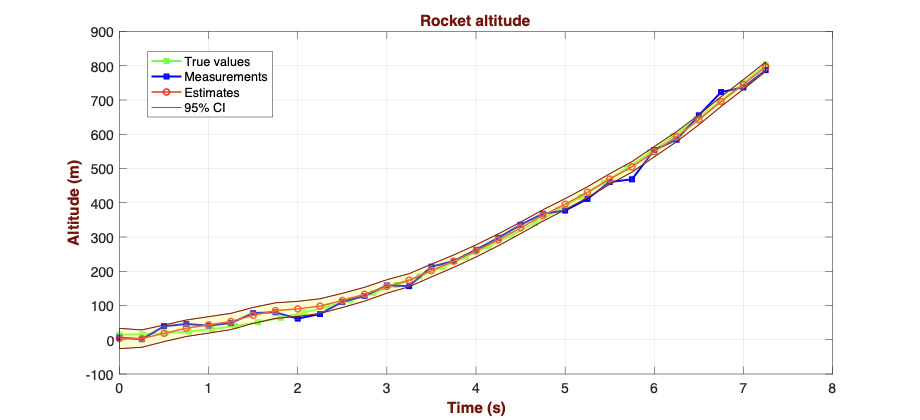
\includegraphics[width=1\linewidth]{Figures//Chapter3/Ex10_RocketAltitude.png}
    \label{fig:enter-label}
\end{figure}
\vspace{-10pt}
\begin{figure}
    \centering
    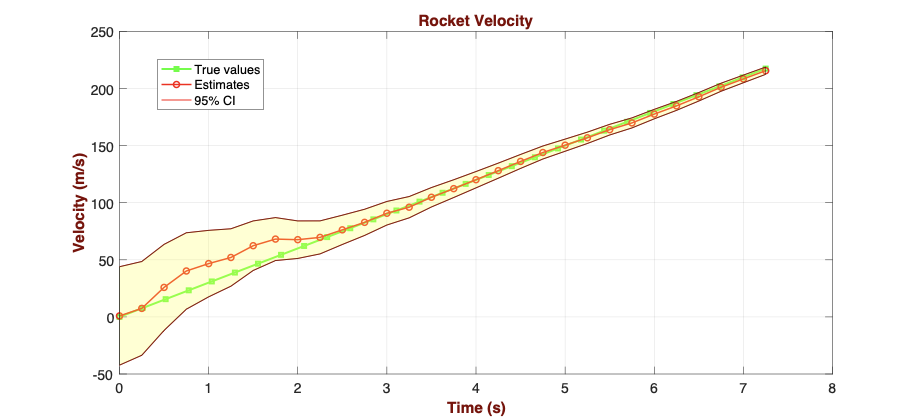
\includegraphics[width=1\linewidth]{Figures//Chapter3/Ex10_RocketVelocity.png}
    \label{fig:enter-label}
\end{figure}


\end{columns}
\texttt{\tiny [Code: Multivariate KF/ex10\_MultivariateKF\_RocketAltitudeEstimation.m]}
\end{frame}